\documentclass[a4paper,10pt,openany,oneside]{report}

\usepackage{amsfonts}
\usepackage{amsmath}
\usepackage{amssymb}
\usepackage[french]{babel}
\usepackage{changepage}
\usepackage{color}
\usepackage{enumitem}
\usepackage{fancyhdr}
\usepackage[T1]{fontenc}
\usepackage[left=3cm,right=3cm,top=3cm,bottom=3cm,headsep=1cm]{geometry}
\usepackage{graphicx}
\usepackage[hidelinks]{hyperref}
\usepackage[utf8]{inputenc}
\usepackage{listings} %Pour le code
\usepackage{titlepic}
\usepackage{wrapfig}
\usepackage{longtable}

\setitemize{topsep=5pt}
\setlength{\parindent}{1em}

\definecolor{dkgreen}{rgb}{0,0.6,0}
\definecolor{gray}{rgb}{0.5,0.5,0.5}
\definecolor{mauve}{rgb}{0.58,0,0.82}
\definecolor{myblue}{rgb}{0,0,1}
\definecolor{bonus}{rgb}{1,0.7,0}

\newcommand\blfootnote[1]{%
  \begingroup
  \renewcommand\thefootnote{}\footnote{#1}%
  \addtocounter{footnote}{-1}%
  \endgroup
}

\lstset{frame=tb,
  language=C++,
  aboveskip=3mm,
  belowskip=3mm,
  showstringspaces=false,
  columns=flexible,
  basicstyle={\small\ttfamily},
  numbers=left,
  numberstyle=\normalsize,
  numbersep=7pt,
  numberstyle=\tiny\color{gray},
  keywordstyle=\color{blue},
  commentstyle=\color{dkgreen},
  stringstyle=\color{mauve},
  breaklines=true,
  breakatwhitespace=true,
  tabsize=4
}

\begin{document}
\begin{titlepage}
\titlepic{
\includegraphics[scale=0.2]{img/iconCB.png}}
\title{City Builder}
\author{Damian Petroff, Sergiy Goloviatinski, Raphaël Margueron}
\date{\today}
\maketitle
\end{titlepage}

%------
\thispagestyle{empty}
\pagebreak
\thispagestyle{empty}
%------
\chapter*{Abstract}
\thispagestyle{empty}
Dans le cadre du "Projet P2", nous, Raphaël Margueron, Sergiy Goloviatinsky et Damian Petroff, avons la tâche de réaliser une application graphique en C++ grâce au framework Qt. 
Ce rapport décrit les étapes de réflexion, conceptualisation et réalisation des différentes facettes du projet. En premier lieu, nous analyserons les besoins du projet et ses spécifications. Ensuite nous détaillerons sa conception, notre planification et notre stratégie de développement. À la suite de quoi nous expliquerons la phase de développement en détail. Enfin, nous proposerons un bilan du projet suivi d'une conclusion traitant de notre ressenti par rapport à cette expérience.
\pagebreak
%------
\thispagestyle{empty}
\tableofcontents
\thispagestyle{empty}
%------
\chapter*{Introduction}
\setcounter{page}{1}
\paragraph{}
L'industrie vidéo-ludique est aujourd'hui un marché grandissant de manière notoire et notre intérêt pour les diverses facettes que ce domaine propose a inévitablement influencé notre choix.
En effet, la conception d'un jeu-vidéo n'est de loin pas une mince affaire. Dans ce rapport nous allons présenter comment nous avons relevé le défi et notre approche sur sa conception et sa réalisation.

Il est nécessaire de prendre note qu'aucun de nous trois n'avait réalisé ni même conceptualisé de jeu-vidéo auparavant, malgré cela, c'est un domaine très intéressant et très complet qui laisse part à la créativité autant sur le plan artistique que scientifique du fait de la diversité des corps de métier nécessaires à l'élaboration d'un tel produit. Le dessin, la sculpture, l'architecture, la musique, la littérature et le cinéma sont quelques uns des arts présents dans la conception d'un jeu-vidéo et nous sommes trois développeurs possédant peu de connaissances en création de contenu audiovisuel, il est donc évident que nous nous sommes orienté vers un jeu de type réflexion ou gestion, qui contient relativement beaucoup d'algorithmie. Le but n'étant pas non plus de créer un sudoku.

\paragraph{Vers un city builder :}
L'idée d'un jeu portant sur la conception et la gestion d'une ville nous a paru appropriée, chacun de nous connait un tant soit peu le sujet, ayant joué à des grosses licences comme "\textit{Cities: Skylines}" de Colossal Order\footnote{Colossal Order : \textcolor{blue}{\url{www.colossalorder.com}}}
\blfootnote{\hspace{7pt}Figure 1. Source de l'image : \href{https://www.reddit.com/r/CitiesSkylines/comments/3mubt5/finally_my_first_city_in_more_then_80_hours_i/}{\texttt{\textcolor{blue}{www.reddit.com/r/CitiesSkylines}}}}
 ou encore "\textit{SimCity}" de Electronics Arts\footnote{Electronics Arts : \textcolor{blue}{\url{www.ea.com}}} pour ne citer qu'elles. Ce type de jeu de gestion laisse place à une certaine liberté de contenu (comme les bâtiments disponibles, les ressources nécessaires, etc.). Nous avons donc pris la décision de créer un produit de la même nature, en version extrêmement plus modeste évidement.
\begin{center}
	\begin{figure}[h]
	\centering
	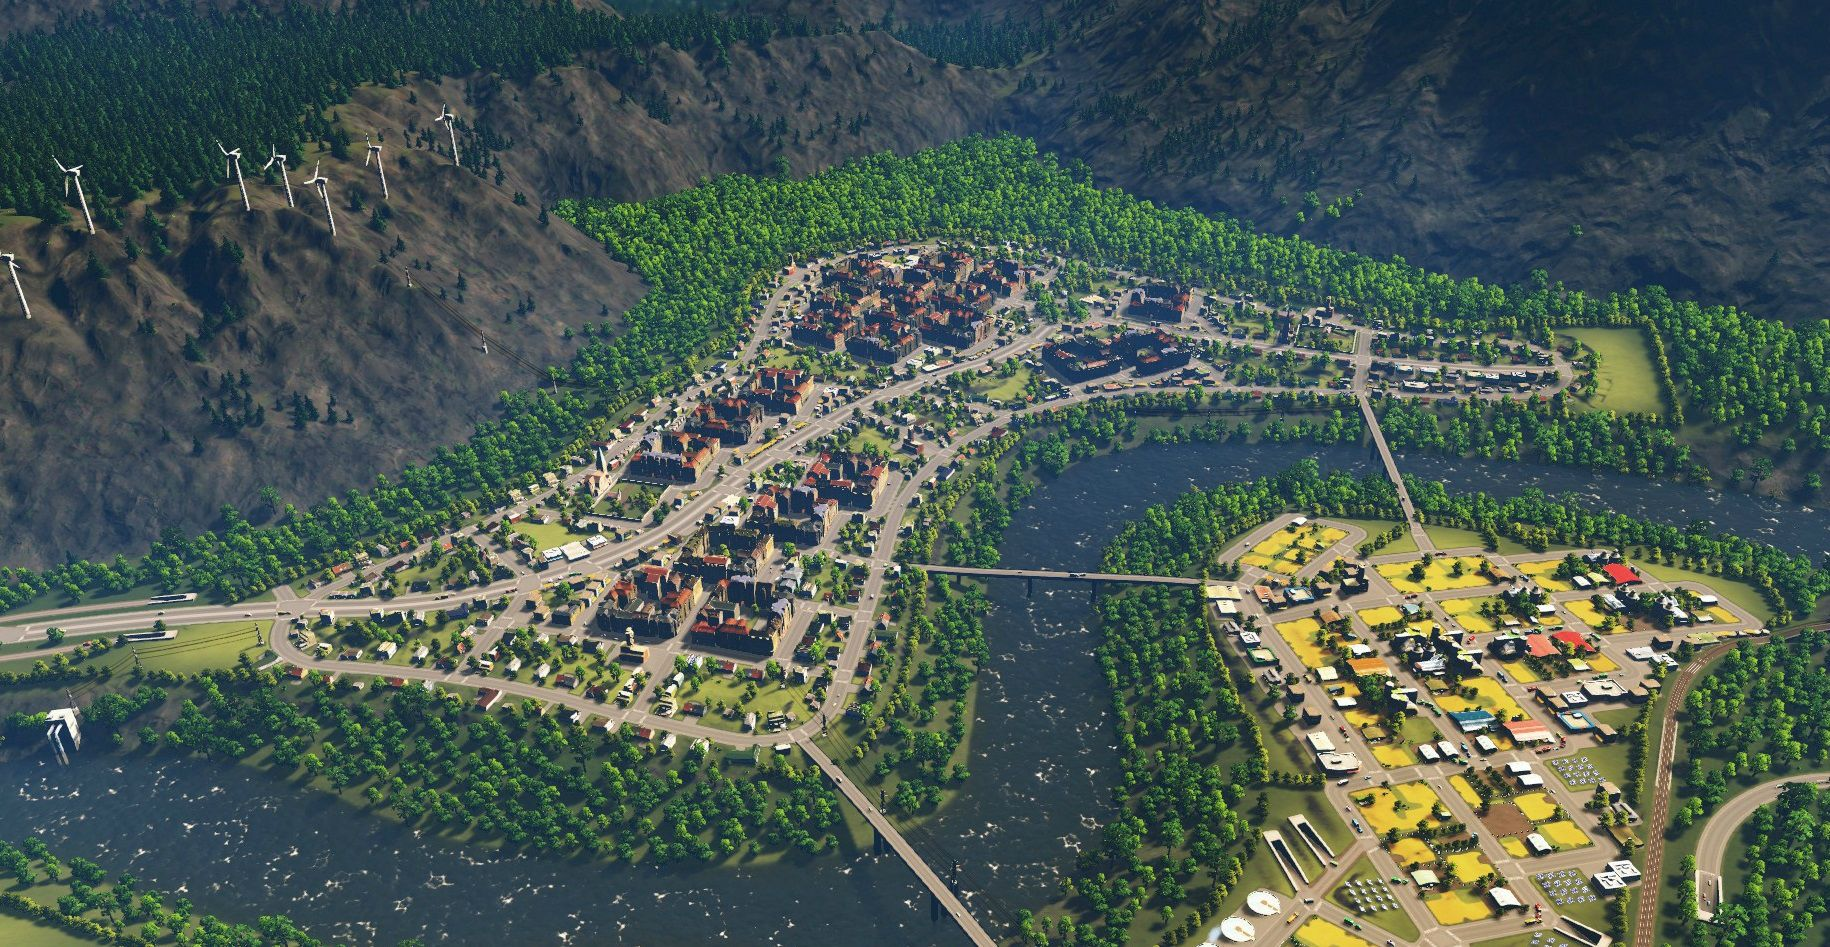
\includegraphics[width=0.9\textwidth]{img/img_intro_cscity.jpg}
	\caption{\label{fig:Cities: Skylines city}Un village sur Cities : Skylines}
	\end{figure}
\end{center}

\thispagestyle{empty}
\paragraph{}
Le but principal du projet est de produire un city builder avec des interactions basiques, un certain panel d'actions possibles rendant le jeu "jouable" et significativement unique. L'application doit être stable et répondre aux spécifications (cf. section 1.1 Spécifications). Le joueur a la possibilités de commencer une nouvelle partie avec des paramètres personnalisés et de reprendre une partie déjà commencée (principe de sauvegarde). L'application doit être codée en C++ via le framework Qt qui permet de faciliter l'affichage et la gestion des éléments graphiques et des conteneurs. Les éléments du framework Qt appris au cours aident à concevoir les composants graphiques principaux nécessaires.

\chapter{Analyse des besoins}
\thispagestyle{headings}
\section{Exigences fonctionnelles}
\subsection{Spécifications}
Voici les spécifications principales\footnote{Par spécifications principales, on entend les fonctionnalités nécessaires, sans citer celles bonus, qui viendront à la section suivante} du projet :
\subsubsection{Général}
\begin{itemize}
\item Possibilité de créer une nouvelle partie avec des paramètres personnalisés comme :
\begin{itemize}
\item La taille de la carte;
\item La difficulté;
\item Le nom de la partie.
\end{itemize}
\item Possibilité de charger une sauvegarde d'une partie
\item Le jeu est en plein écran
\item Utilisation de contenu audio (musique d'ambiance, événements)
\item Possibilité de voir toute la carte à la fois ou alors de zoomer puis de se déplacer en haut, en bas, à gauche et à droite
\item La carte est divisée en cases carrées, certains bâtiments peuvent utiliser plusieurs cases
\end{itemize}
\subsubsection{Mécaniques de gameplay}
L'application doit permettre de :
\begin{itemize}
\item construire des routes;
\item construire des habitations;
\item construire des bâtiments publics qui ont un effet sur la population;
\item voir le rayon d'effet d'un tel bâtiment lors de sa construction;
\item détruire des éléments déjà construits;
\item construire un élément qu'à condition d'en avoir les moyens financiers;
\item construire un élément qu'à condition d'avoir déjà construits le ou les éléments requis à sa construction (exemple : Construire une tour Eiffel ne peut se faire que dans un ville relativement grande.)
\item créer une économie via des coûts de certaines infrastructures;
\item gérer les frais imposés aux habitants ;
\end{itemize}

\subsubsection{Interface utilisateur}
Le HUD\footnote{\textit{Head Up Display} : Communication graphique des informations avec le joueur} du jeu comporte :
\begin{itemize}
\item L'affichage de plusieurs indicateurs étroitement liés représentant la ville
	\begin{itemize}
		\item L'argent (représente les caisses de la ville)
		\item Le bonheur (représente la satisfaction des habitants par rapport à la ville)
		\item La population (représente la quantité d'habitant dans la ville)
	\end{itemize}
\item Un menu d'options, sauvegarde, quitter la partie, etc.;
\item Le carte en elle-même;
\item Un onglet de construction de bâtiments;
\end{itemize}

\subsubsection{Rendu graphique}
\begin{itemize}
\item Le jeu est en 2.5D (2D isométrique)
\item Une différence visuelle entre terrain constructible et non-constructible
\item Une différence visuelle entre les différents types de bâtiments, via des couleurs par exemple.
\end{itemize}

\subsubsection{Bâtiments}
Le panel de bâtiments doit être relativement complet et toucher à plusieurs domaines comme :
\begin{itemize}
\item \textbf{La santé : }clinique, hôpital, cimetière, crématoire, sauna, laboratoire médicaux, dépôt pour hélicoptère médical, etc.
\item \textbf{Les services d'urgence : }caserne de pompier, dépôt pour hélicoptère de pompier / Canadair, tour de garde, unité de réponse en case de catastrophe, bunker, antenne radio, etc.
\item \textbf{L'éducation : }école primaire, école secondaire, école professionnelle, lycée, université, faculté, etc.
\item \textbf{Les transports : }dépôt de bus, station de bus, arrêt de bus, pareil pour tram, métro, taxi, train, bateau, avion, etc.
\item \textbf{Les loisirs : }restaurant, centre commercial, bibliothèque, parc, place de jeu, jardin botanique, parc d'attraction, terrain de sport, lieu de pêche, étable, skate park, etc.
\item \textbf{Les monuments : }stade de foot, Tour Eiffel, statues, mémoriaux, fontaines, etc.
\end{itemize}

\subsubsection{Ressources dans le jeu}
\begin{itemize}
\item Argent
\end{itemize}

\subsubsection{Bonheur des citoyens}
Le bonheur des citoyens est généré grâce aux infrastructures et aux services qui leur sont proposés dans une portée donnée, par exemple :
\begin{itemize}
\item Un supermarché;
\item Un hôpital;
\item Un poste de police;
\item Une école;
\item Un arrêt de bus;
\item Un lieu de loisir;
\item Un monument.
\end{itemize}
Certains éléments peuvent affecter négativement le bonheur comme des impôts trop élevés, avoir un manque d'accès à un hôpital, etc. 

\subsubsection{Croissance de la population}
La croissance de la population doit avoir un sens et être en accord avec le nombre de bâtiments présents et le bonheur des citoyens. 


\subsection{Spécifications bonus}
Cette section tient d'indication sur quelques idées que nous avions au cas où le temps nous le permettrait.

\subsubsection{Général}
\begin{itemize}
\item Possibilités de générer des cartes aléatoirement avec des lacs, montagnes, etc.
\item Pré-visualisation de la carte à générer;
\end{itemize}

\subsubsection{Mécaniques de gameplay}
\begin{itemize}
	\item Impossible de construire un bâtiment sans route qui le borde
	\item Filtre pour afficher la quantité de bonheur apportée par case (somme des effets de tous les bâtiments). Permet de savoir quelles sont la zone la plus ou moins heureuse de la ville.
	\item Système de quêtes pouvant servir de tutoriel, par exemple:
	\begin{itemize}
		\item Construire une route
		\item Construire quatre maisons
		\item Récompense : 200 \$ et déblocage d'un bâtiment
	\end{itemize}
	\item Gérer plusieurs difficultés
	\item L'évolution de la population en fonction du bonheur et du temps (flux migratoires), par exemple : Le nombre d'habitants au sein d'une habitation augmente au fil du temps.
	\item Les événements aléatoires.
\end{itemize}

\subsubsection{Interface utilisateur}
\begin{itemize}
\item Une minimap affichable ou non sur laquelle il serait possible de cliquer pour se rendre au bon endroit directement
\end{itemize}

\subsubsection{Rendu graphique}
\begin{itemize}
\item Nos propres textures de bâtiments et de routes grâce auxquelles il serait possible de créer un thème comme le futurisme, le western ou même une ville technologiquement évolutive dans le temps
\item Textures adaptatives des routes, gestion des virages et des croisées
\item Temps de construction d'un bâtiment, sous forme d'un chantier animé
\item Animations. Par exemple, bonshommes qui marchent dans la rue et voiture qui roulent sur les routes.
\item Cycles jour / nuit.
\end{itemize}

\subsubsection{Bâtiments}
\begin{itemize}
\item Les bâtiments peuvent occuper des cases de manière non-rectangulaire (en L par exemple)
\end{itemize}

\subsubsection{Ressources dans le jeu}
\begin{itemize}
\item Électricité
\item Eau
\end{itemize}

\section{Exigences non-fonctionnelles}
\subsection{Codage}
Nous avons choisi d'utiliser le design pattern $singleton$ pour toutes nos classes gestionnaires qui devaient être appelées depuis plusieurs endroits, ceci pour éviter de devoir les mettre comme attributs dans toutes les autres classes.
\subsection{Portabilité}
Nous avons décidé de porter le jeu sur les plateformes utilisés par les membres du groupe, à savoir Windows et Linux
\subsection{Ergonomie}
Les interactions sont simples et malgré les quelques bugs possibles, la gestion de la ville est relativement facile à prendre en main lorsque le joueur a quelques minutes de jeu à son actif.
\subsection{Efficience}
\subsubsection{Temps de réponse}
Dans notre cas, le temps de réponse n'est pas une contrainte essentielle car nous n'utilisons pas de communication réseau et le jeu ne se repose pas sur la réactivité mais plutôt sur la réflexion. En revanche, pendant les chargement et générations de parties, nous notifions le joueur qu'un chargement a lieu afin de le rassurer.
\subsubsection{Utilisation des ressources}
Le jeu ne se veut pas trop "lourd" et tourne aisément sur une machine standard actuelle.
\subsection{Maintenabilité}
Grâce à une bonne modularisation des classes, la compréhension, la maintenance et l'amélioration du code de l'application est relativement simple.
\section{Cas d'utilisation}
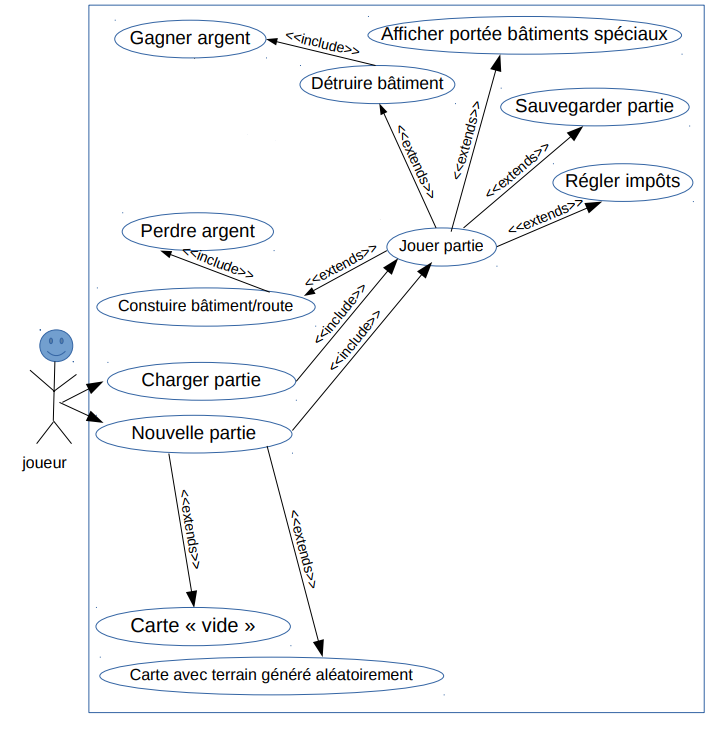
\includegraphics[width=\textwidth]{img/usecase.png}

\chapter{Conception}
\thispagestyle{headings}
\section{Stratégie de conception}
\subsection{Planification initiale}
\paragraph{}
Voici note planning initial :
\begin{center}
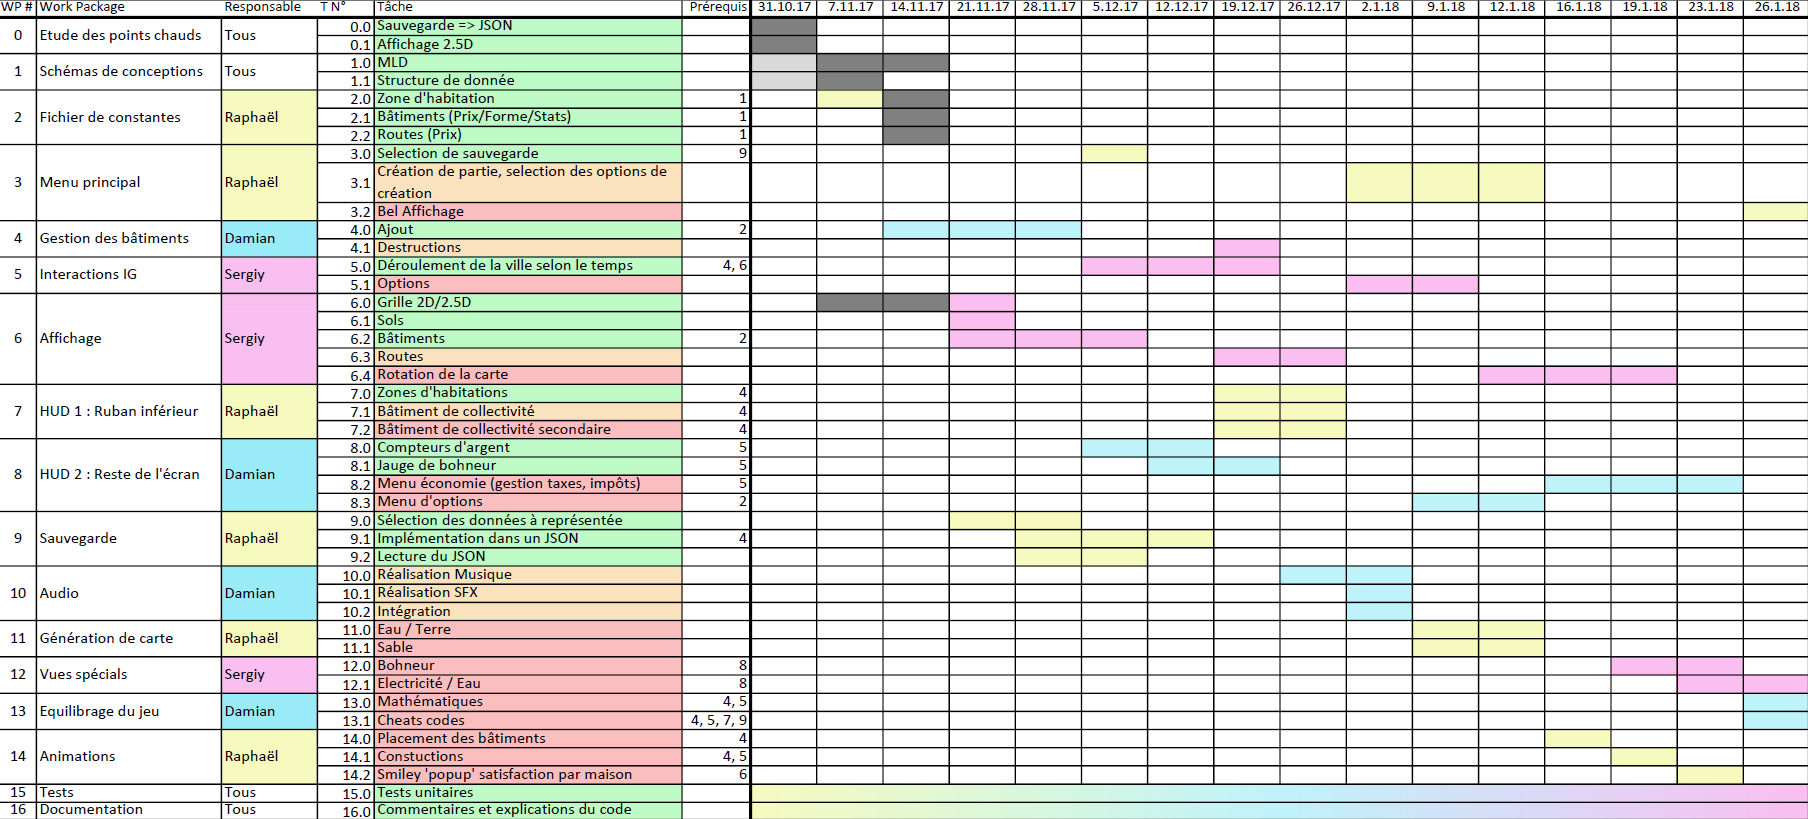
\includegraphics[width=1.1\textwidth]{img/planning_initial.png}
\end{center}
\subsection{Architecture logicielle}
\subsubsection{Schéma procédural}
\begin{center}
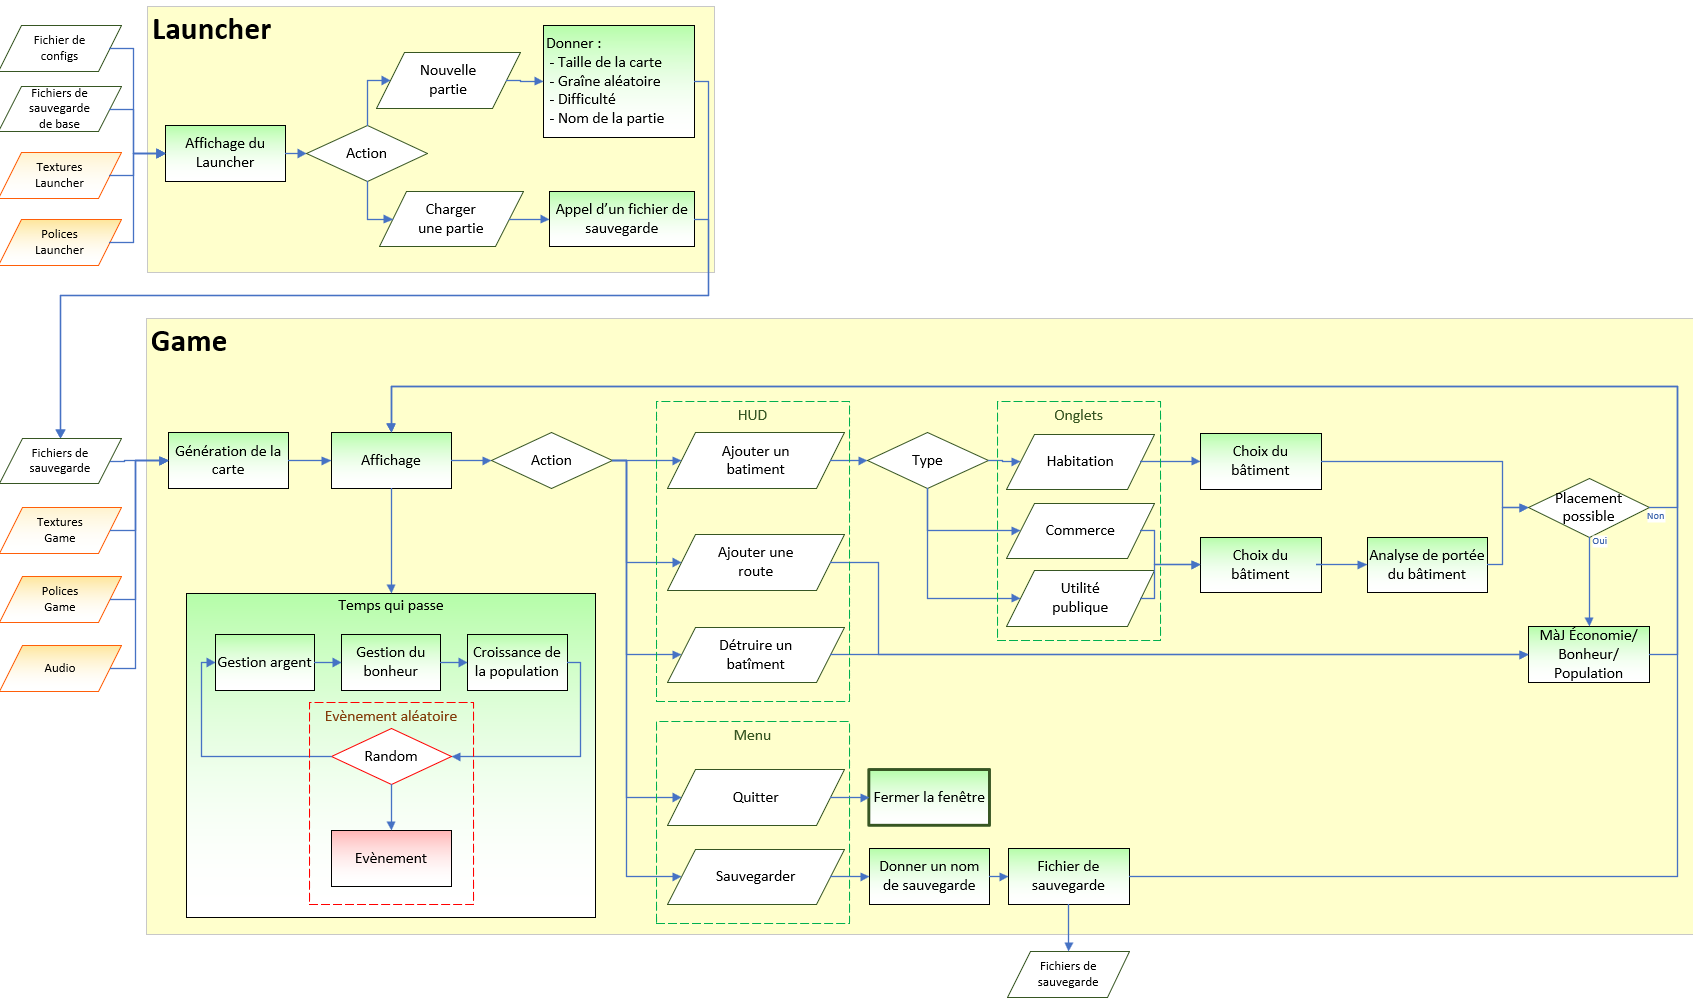
\includegraphics[width=\textwidth]{img/schema_proc.png}
\end{center}
Le bloc en rouge n'a pas été implémenté
\subsubsection{Diagramme de classe}
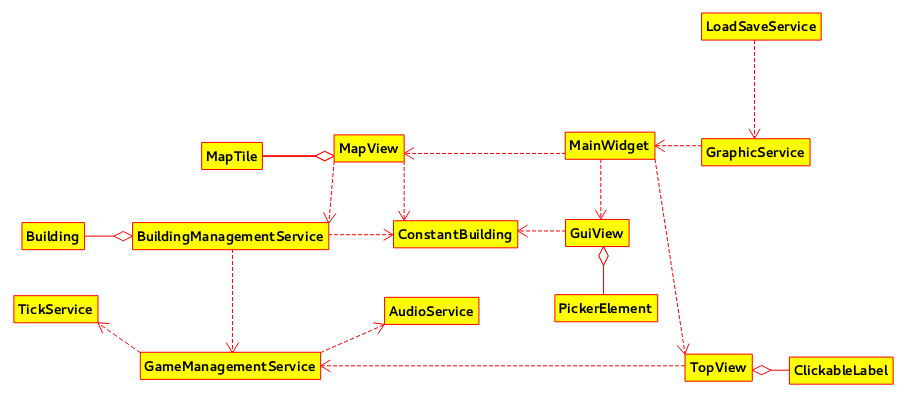
\includegraphics[width=0.9\textwidth]{img/hierarchieClasses.png}
\begin{itemize}
\item Le point d'entrée est $LoadSaveService$, qui soit charge une sauvegarde ou soit crée une nouvelle partie à partir des arguments passés au $main$
\item $GraphicService$ comporte des méthodes généralistes utilisés par toutes les vue comme par exemple la gestion des raccourcis claviers ou la coloration des bâtiments selon leurs catégorie
\item $GuiView$ contient l'interface utilisateur qui permet de poser des routes/bâtiments ou les détruire (se trouve en bas de l'écran), les boutons de ce menu sont représentés avec la classe $PickerElement$, quand on clique sur un $PickerElement$ (autre que ceux représentant les catégories) la $MapView$ se mets dans le mode correspondant
\item $TopView$ contient l'interface utilisateur qui nous montre les informations sur la partie et permet de faire divers configurations (volume musique, niveau des taxes p. ex) et actions  (charger/sauvegarder partie p. ex)
\item $MapView$ contient l'affichage du terrain de jeu, et est composé de $MapTile$ qui représentent les cases du jeu
\item $ConstantBuilding$ stocke les informations sur les bâtiments (nom, catégorie, prix, portée d'effet, etc.)
\item $BuildingManagementService$ gère la logique des bâtiments, c'est à dire le calcul du prix, du bonheur, la gestion des portées d'effets etc. , de plus contient les structures de données contenant les $Building$ qui sont des bâtiments qui ont été instanciés au cours de la partie
\item $GameManagementService$ gère la logique "haut niveau" du jeu, donc contient les valeurs sur l'argent, le bonheur et la population, et s'occupe d'instancier le $TickService$ et $AudioService$
\item $TickService$ recalcule les données du jeu s'il y a eu un bâtiment ajouté/retiré depuis le dernier tick, un tick s’exécutant chaque seconde
\item $AudioService$ est appelé pour jouer la musique du jeu, et pioche parmi plusieurs sons possibles à chaque fois qu'on construit un bâtiment
\end{itemize}
\subsubsection{Convention de codage}
La convention de codage utilisée est celle spécifiée sur la forge\footnote{\href{https://forge.ing.he-arc.ch/gitlab/dgr/Ressources/wikis/convention}{\textcolor{blue}{La forge}}}.
\section{Interface utilisateur}
Cette section traite des choix faits sur les possibilités d'interactions de l'utilisateur avec l'application. En premier lieu sera présenté le launcher, puis le client. 
\subsection{Launcher}
\subsubsection{Esthétique}
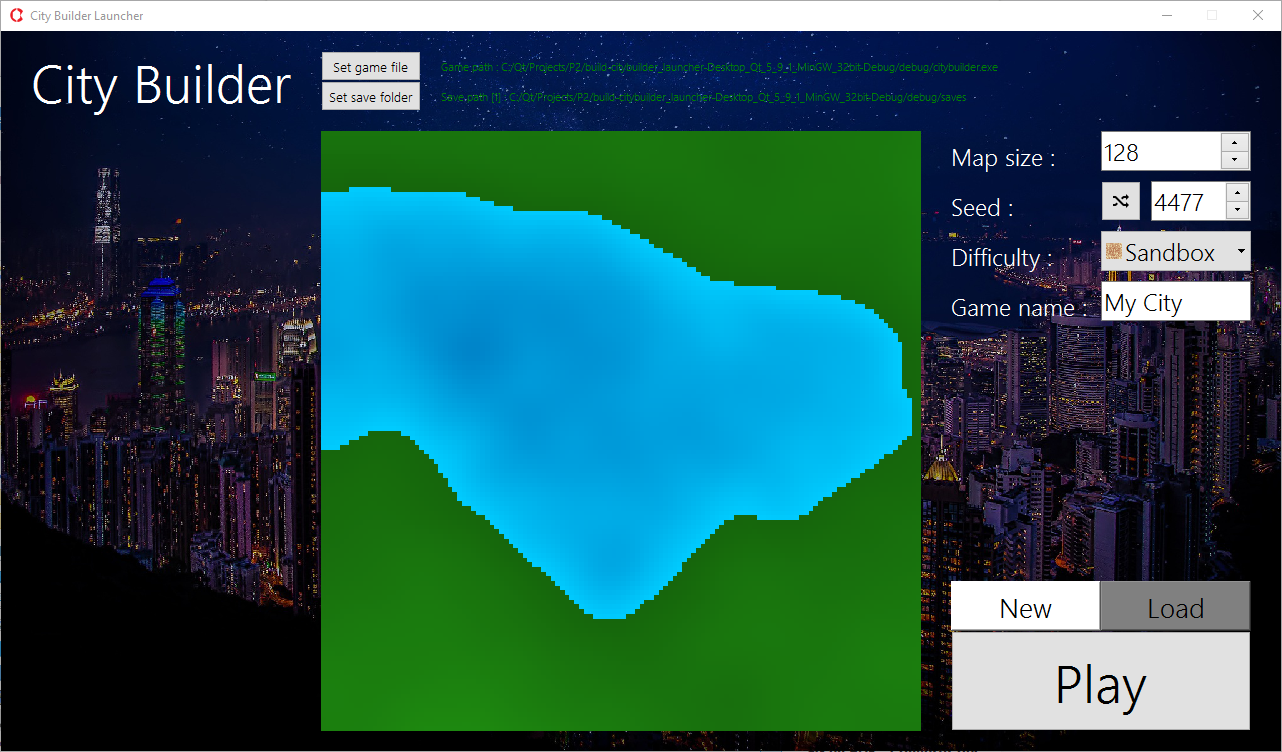
\includegraphics[width=\textwidth]{img/ui_launcher.png}
\subsubsection{Interactions et raccourcis}
\paragraph{}
De manière générale, nous avons opté pour une interaction simple et intuitive. Il y a deux possibilités : Créer un nouvelle partie et en charger un à partir d'une sauvegarde.
\paragraph{}
L'utilisateur doit indiquer l'emplacement de l'exécutable du jeu et l'emplacement du dossier contenant des sauvegardes s'il souhaite en charger une.

\subsection{Client}
\subsubsection{Esthétique}
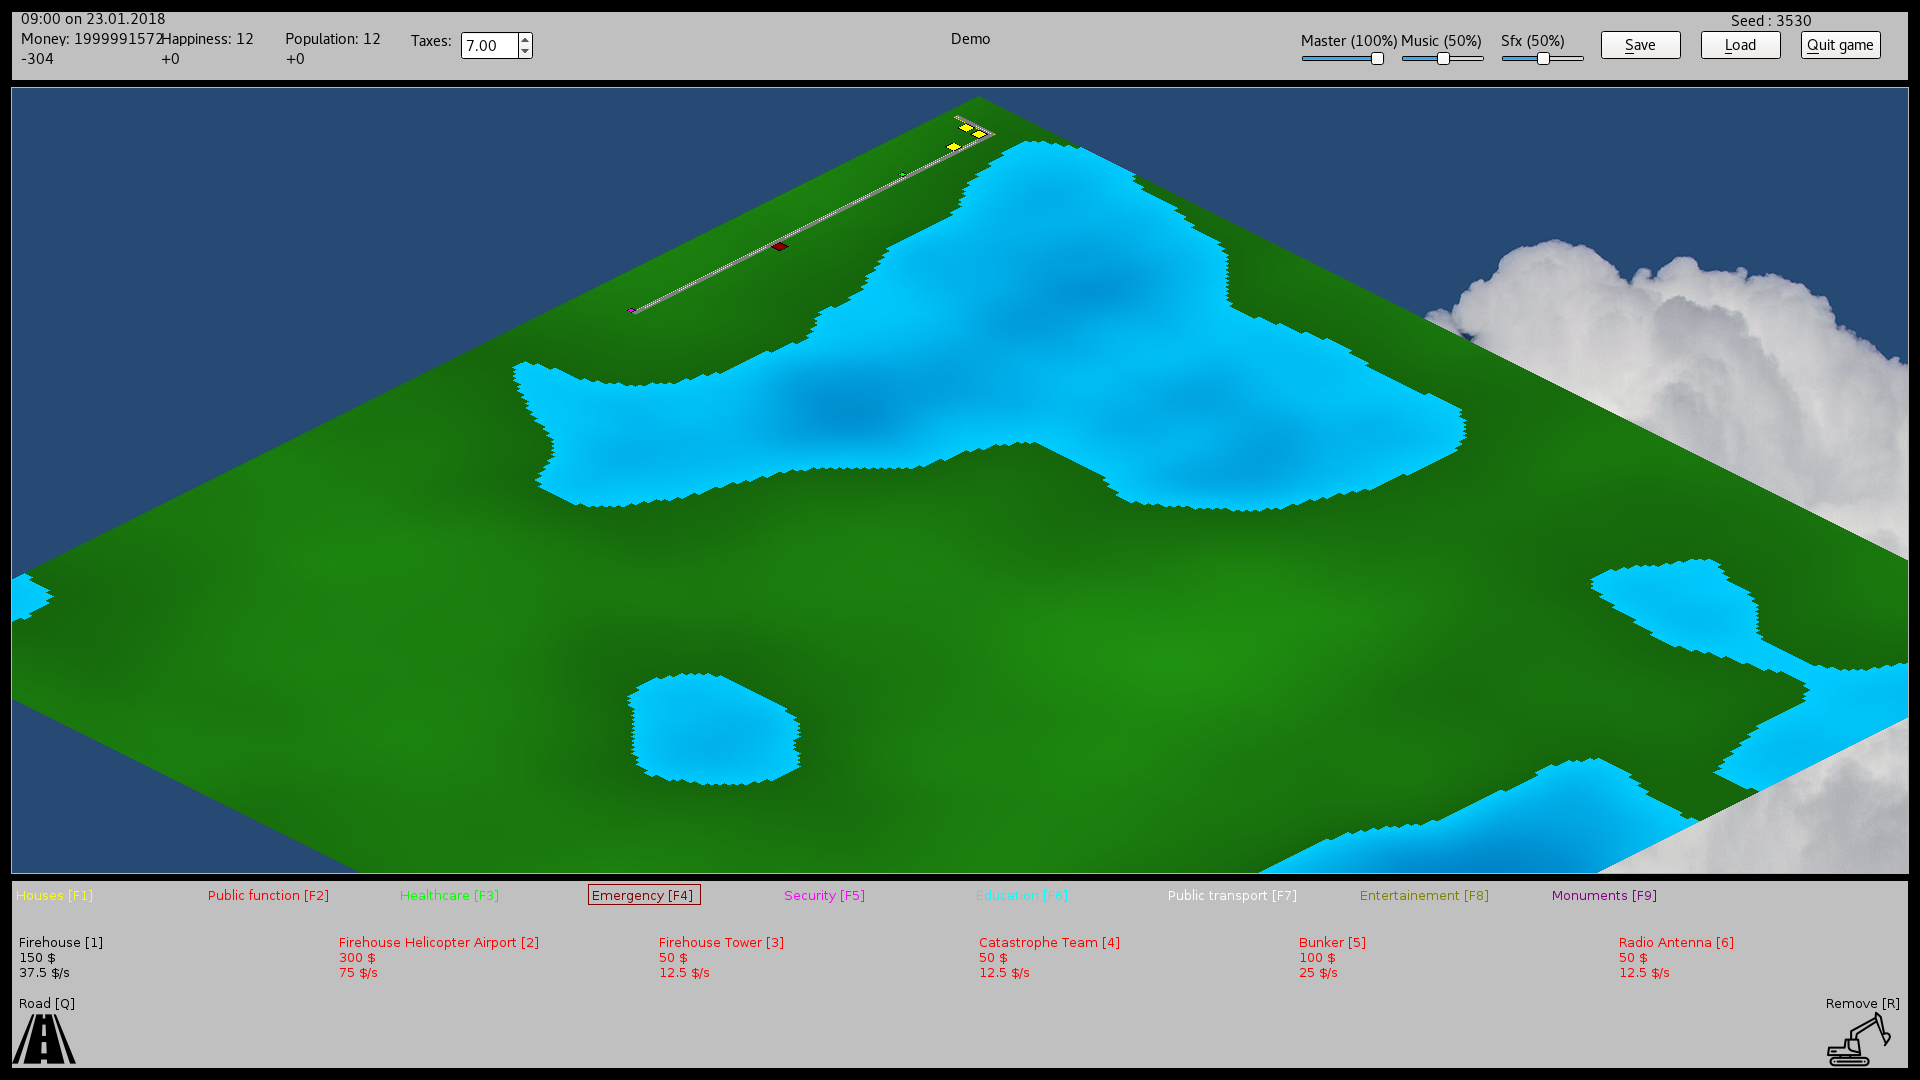
\includegraphics[width=\textwidth]{img/ui_client.png}
\subsubsection{Interactions et raccourcis}
\paragraph{}
L'interface graphique se divise en 3 parties:\\\\
$TopView$ : Vue fixe se trouvant toujours en haut de l'interface et qui contient:
\begin{itemize}
\item L'heure et la date dans le jeu
\item Des indicateurs d'argent, de bonheur et de population disponible pour le joueur avec le delta entre chaque seconde
\item Une $SpinBox$ permettant de régler le niveau d'impôts
\item Le nom de la carte, pouvant être modifié si on clique dessus
\item Des $Slider$ pour régler le volume de la musique et des effets
\item Des boutons pour charger,sauvegarder et quitter la partie
\item La valeur de la seed utilisée pour générer la carte
\end{itemize}
$MapView$ : Contient le terrain de jeu, les différents raccourcis claviers (même quand cette vue n'a pas le focus) et actions de souris qui sont dans son focus influencent sur cette vue:
\begin{itemize}
\item Translation dans la vue (Raccourcis: A S D W ou flèches directionnelles)
\item Zoom dans la vue (Raccourcis : + - ou molette de la souris)
\item Afficher/masquer la grille (Raccourci: G)
\item Afficher/masquer les rayons d'effets de tous les bâtiments qui en ont un (Raccourci: F)
\item Afficher le rayon d'effet d'un bâtiment s'il en a un quand on clique dessus
\end{itemize}
$GuiView$ : Vue contenant les boutons permettant de:
\begin{itemize}
\item Choisir la catégorie de bâtiment à poser (Raccourcis clavier disponible depuis n'importe quelle vue: F1 à F9)
\item Les différents bâtiments à poser selon la catégorie choisie (Raccourcis claviers de 1 à 0)
\item Un bouton pour poser des routes disponibles dans toutes les catégories (Raccourci: Q)
\item Un bouton pour supprimer un bâtiment/route disponible dans toutes les catégories (Raccourci: R)
\end{itemize}





\chapter{Développement et réalisation}
\thispagestyle{headings}
\section{Fonctionnalités du launcher}
Le launcher permet de créer une interface entre les paramètres de création de partie ou le chargement de sauvegarde et les argument en ligne de commande du client.
\subsection{Création d'une partie}
Pour la création d'un partie nous avons réfléchi sur quel paramètre nous laissions libre à l'utilisateur et nous avons développé une interface autour de ceux-ci.
\newline
Les paramètres que nous avons retenu sont les suivants :
\begin{itemize}
	\item La taille de la carte (en case)
	\item La graine de la carte (seed)
	\item La difficulté de la partie (Argent de départ)
	\item Le nom de la ville
\end{itemize}
Étant donné que la taille de la carte et la seed pouvait être précisé lors de la création d'une partie, nous avions tous les paramètres pour offrir à l'utilisateur la pré-visualisation de la carte.
\subsection{Chargement d'une partie}
Pour charger les parties dans l'onglet Load, tous les fichiers .cbsave du dossier de sauvegarde spécifié sont présenté à l'utilisateur. Le dossier peut être changé en cliquant sur le bouton "Save save folder".
Si une sauvegarde est sélectionné et que l'utilisateur appuie sur "Play" le launcher va ouvrir le jeu avec comme seul argument le chemin absolu du fichier de sauvegarde sélectionné. Aucune pré-visualisation n'est actuellement effectué avec les sauvegardes.
\section{Fonctionnalités du client}
\subsection{Génération des sols}
Pour la gestion du terrain, nous avons décidé d'avoir deux types de sol : l'eau et l'herbe. Sur l'herbe, il est possible d'ajouter des bâtiments et sur l'eau non.

Pour pouvoir avoir des cartes auto-générée, nous avons décide d'utiliser un algorithme de bruit de Perlin. Nous n'allons pas aller dans les détails du fonctionnement du bruit de Perlin, dans ce rapport. Mais son principe est le suivant: il permet d'avoir des nombres aléatoires qui sont proche les uns de autres en function d'une seed(pour l'aléatoire, initialisé au début) et de 1, 2 ou X dimensions (trois dans celui que nous avons utilisés, mais que 2 utilisés). Vu que les outputs de la function de bruit de Perlin sont les mêmes quand nous utilisons les mêmes inputs. Nous pouvons la considérer comme une fonction à plusieurs variables (qui sont les dimensions et la seed). Changer la seed donne des résultats complètement différent mais changer les autres variables change peu entre chaque valeur.

\[bruit = perlin(seed, x, y, z)\]

Les nombres aléatoires que nous récupérons de la function sont des nombres flottant entre 0 et 1.
Leurs distribution sont sous la forme d'une distribution normal, avec un écart type de 1 et .
\[y=e^{-x^{2}}\]

Pour pouvoir générer la carte nous parcourons toutes les cases de la carte (selon x et y). Et "nous déplaçons sur le fonction de Perlin" d'un certain offset (qui est un multiple des index des cases). \\
On calcule la le bruit de Perlin sur cette case et si la valeur valeur est entre 0.3 et 0.7 la case est une case d'herbe. Sinon c'est une case d'eau. \\
Pour pouvoir obtenir un dégradé dans les couleurs de la carte nous somme nous avons converti la tranche du type de case (Eau : 0.0-0.3 ou 0.7-1.0, Herbe : 0.3-0.7) vers les valeurs RGB suivante :
\begin{itemize}
	\item Herbe :
	\begin{itemize}
		\item R : 22 - 39
		\item G : 102 - 178
		\item B : 12 - 21
	\end{itemize}
	\item Eau :
	\begin{itemize}
		\item R : 0 - 0
		\item G : 0 - 204
		\item B : 102 - 255
	\end{itemize}
\end{itemize}
\subsection{Gestion des cases de la carte}
Nous stockons les cases de la carte dans un $QArray$ d'une longueur $nbCases^{2}$

Une case à la coordonnée $X;Y$ dans la grille de cases représentant la carte correspond à l'élément se trouvant à l'indice $X+Y nbCases$ dans le $QArray$

Une case de la carte est représenté par la classe $MapTile$ dérivé de la classe $QGraphicsRectItem$ et contient les attributs suivants:
\begin{itemize}
\item bOccupied (boolean): dit si la case est occupée par un bâtiment ou de l'eau ou pas
\item x (int): coordonnée en x dans la matrice contenant les MapTile
\item y (int): coordonnée en y dans la matrice contenant les MapTile
\item bId (int): id du type de bâtiment (tous les hôpitaux ont la même bId p. ex)
\item unique BId (int): id unique du bâtiment (chaque bâtiment posé aura une id unique différente)
\item mainTileX (int): coordonnée en X de la case principale (en haut à gauche), utile pour les bâtiments d'une largeur ou hauteur supérieures à 1
\item mainTileY (int): même chose que mainTileX mais la coordonnée Y
\item buildingWIdth (int): largeur en nombre de cases d'un bâtiment
\item buildingHeight (int): hauteur en nombre de cases d'un bâtiment
\item bPix (boolean): indique si la case a une texture ou pas
\item buildImage ($QGraphicsPixmapItem*$): Pointeur vers la texture du bâtiment/route qui se trouve sur la case
\end{itemize}
\subsection{Routes et bâtiments}
Pour la gestion des routes et des bâtiments nous sommes parti sur une approche plutôt simple qui est d'avoir divisé en trois classe qui chacune des rôles spécifique. Une qui décrit les caractéristiques propre à chaque bâtiments : les constantes -> ConstantBuilding. Une seconde classe qui décrit une bâtiment spécifique à la partie -> Building. Et une troisième qui sert de gestionnaires de building, 'classe tableau' -> BuildingManager. 

\subsubsection{Constant Building}
Constant Building contient une function de construction d'un tableau d'objet de 'soit même'. Chacun de ces objet représente un bâtiment avec toutes ces caractéristiques internes, par exemple : le prix de construction, la liste des bâtiments nécessaires pour sa construction ou encore sa catégorie dans l'affichage de l'HUD.

Liste de caractéristique de base de chaque bâtiment :
\begin{itemize}
	\item Nom à l'affichage
	\item Catégorie
	\item Prix
	\item Largeur (au sol)
	\item Hauteur (au sol)
	\item Une liste de case ignoré (non-implémenté, pour avoir la possibilité d'avoir de bâtiment non rectangulaire)
	\item Type de pré-requis (Ou / Et)
	\item Une liste d'identifiant de bâtiment pré-requis.
	\item La sommes des pré-requis nécessaires. 
\end{itemize}

Nous avons choisi d'avoir des objets au lieu d'une liste de constante, pour pouvoir avoir la possibilité d'y ajouter des fonctions pour ces objets ce qui nous a permis d'avoir un autre set de valeur basé sur les caractéristiques de base, voir ci-dessous. Cela nous permet ajuster facilement le jeu et d'avoir une sorte de progression linaire du jeu.

Liste des caractéristique dérivé :
\begin{itemize}
  \item Prix/Secondes = \(Prix / 4\)
  \item Efficacité = \((Prix/10)^{1.4} + 10\) (arrondi au multiple de 25 le plus proche)
  \item Rayon d'action = \(Log10(PrixParSecondes*Efficacite + 1)\) (Arrondi au multiple de 5 le plus proche)
  \item Poids du Bâtiment dans les pré-requis = \(Prix / 10\)
\end{itemize}

On remarque donc que le prix du bâtiment influe directement sur tous les caractéristique qui définisse si le bâtiment est performant ou non.

Fonctionnement des pré-requis :
Les pré-requis sont un aspect que nous considérons comme l'élément primordiale permettant au jeu d'avoir une progression. Le principe est le suivant.

Pour qu'un bâtiment soit accessible à la construction il faut qu'il respect les règles suivantes si son type de pré-requis est 'ou' :
La somme des poids de tous les bâtiments qui sont actuellement posé qui sont dans la liste des bâtiments en pré-requis du bâtiment désiré doit être supérieur ou égal à la somme des pré-requis nécessaires.
Exemple :
Pour poser un Laboratoire médical : Il faut au moins une somme de 6.
La liste des bâtiments pré-requis et des poids pour le laboratoire est la suivante :
\begin{itemize}
	\item Clinique : 1
	\item Hôpital : 5
\end{itemize}
Il y a donc au moins trois possibilités pour arriver à remplir cette demande :
\begin{itemize}
	\item 6x Clinique
	\item 1x Clinique et 1x Hôpital (Meilleur solution, au niveau du prix par seconde de le efficacité sur un grand rayon)
	\item 2x Hôpital
\end{itemize}

Pour les pré-requis en 'et' :
Il faut en plus que pour les pré-requis en 'ou', avoir au moins un bâtiment de chaque type de la liste des bâtiments pré-requis.
Exemple :
Pour poser une Tour Eiffel : Il faut au moins une somme de 11.5
La liste des bâtiments pré-requis et des poids pour le laboratoire est la suivante :
\begin{itemize}
	\item Hôpital : 5
	\item Caserne de pompier : 1.5
	\item Quartiers généraux : 5
\end{itemize}
Il y a donc au moins une possibilité pour arrivé à remplir cette demande, qui est d'avoir une bâtiment de chaque. A noter que dans ce cas, la somme de pré-requis n'influence pas pour ce bâtiment, mais on pourrai imaginer qu'un bâtiment aille une somme plus grande que la somme de chaque bâtiment pré-requis et la la somme aurai une influence.

\subsubsection{Building}
La classe building décrit un bâtiment posé dans une partie. Il est décris les caractéristiques suivantes :
\begin{itemize}
	\item Un identifiant unique
	\item Un identifiant du type de bâtiment (de ConstantBuilding)
	\item Une position X/Y
	\item Un angle de rotation (De quel côté est posé le bâtiment, non-implémenté)
	\item Une population
\end{itemize}
On peut donc noter que cet objet est rendu assez 'léger' car la plus part de ce qui le décrit est géré par l'identifiant constant building. Nous pouvons donc avoir beaucoup de bâtiment et avoir une emprunte mémoire peu conséquente.

\subsubsection{Building Manager}
Cette classe permet de gérer une liste de bâtiment de la classe Building. On peut exécuté les actions suivante :
\begin{itemize}
	\item Ajouter un bâtiment (qui est ajoutable selon les pré-requis)
	\item Supprimer des bâtiments 
	\item Récupérer la population total de la ville.
	\item Récupérer le bonheur moyen de la ville.
	\item Récupérer la somme des prix par seconde.
\end{itemize}

Les fonctions de récupération retournent un valeur stocké mais la valeur stock est recalculé si le besoin l'est, par exemple le bonheur moyen ne varie pas selon le temps mais si un nouveau bâtiment est placé on doit donc recalculer le bonheur moyen.
\subsection{Sélecteur pour poser/détruire route/bâtiment}
Quand on choisi d'ajouter/détruire une route/bâtiment, la $MapView$ se mets en mode "picker" (sélecteur) pendant lequel les cases de la carte se trouvant sous la souris montre un aperçu de l'action choisie:
\begin{itemize}
\item Quand on a choisi l'ajout d'un bâtiment, les cases sous la souris se colorient de la couleur du futur bâtiment quand le placement sous ces cases est possible, disparaît si ce n'est pas possible (quand on mets la souris par dessus un bâtiment déjà existant par exemple), et quand on fait un clique gauche quand les cases sous la souris sont coloriés (donc quand le placement est possible), le bâtiment est effectivement ajouté et devient persistant sur la carte
\item Quand on choisi l'ajout d'une route, la case sous la souris devient grise quand le placement est possible, un premier clic commence à "tirer" la route dans n'importe quelle des 4 directions par rapport à la première case, dés qu'on a choisi une 2ème case, cette direction est "bloquée" et on ne peut que continuer de "tirer" la route dans cette direction, après avoir fini de "tirer" la route un clique gauche de la souris ajoute la route de façon définitive
\item Quand la destruction d'un bâtiment/route est sélectionné, les bâtiments/routes qui se trouvent sous la souris se colorient en noir quand on passe dessus, et un clique gauche dessus supprime le bâtiment/route de la partie
\item Un clique droite pendant ces 3 actions ci-dessus annule l'action en question
\end{itemize}
\subsection{Adaptation des textures de routes dynamique}
Quand on pose une route et que celle-ci a des cases adjacentes avec une route existante, les textures des cases se mettent à jour afin de prendre en compte des éventuelles intersections entre l'ancienne et la nouvelle route (Une case peut devenir un virage, un croisement "en X" ou une intersection "en T")
\subsection{Représentation des bâtiments}
L'idée initiale était d'avoir une texture différente pour chaque bâtiment, mais n'ayant pas trouvé de textures satisfaisantes nous avons juste un bâtiment et les routes qui sont dotés de textures.
\newline
Les autres bâtiments sont des carrés de couleur, avec une couleur unique par catégorie de bâtiment (de toutes façons pour le calcul de bonheur l'important c'est d'avoir un bâtiment de chaque type et la distance séparant une maison d'un bâtiment à effet)
\subsection{Déroulement en fonction du temps de la partie}
Le jeu se déroule en fonction du temps sur divers aspects, cela permet d'avoir une progression. Toute les secondes certain calcules sont effectuer pour donner l'impression au joueur que le temps défile. Voici les trois indicateurs que nous avons choisis de représenté :
\begin{itemize}
	\item Bonheur : Représente une satisfaction de la population sur la ville construite.
	\item Argent : Le solde que la ville a à disposition pour faire de modifications.
	\item Population : Le nombre d'habitant qui réside actuellement dans la ville.
\end{itemize}
Malgré nos efforts à rendre le jeu jouable. Nous avons parfaitement conscience que le jeu n'est pas très bien équilibré à ce niveau.
\subsubsection{Temps : Heure et Date}
Pour pouvoir donner un aspect réaliste au jeu, nous avons choisi de prendre la date du jour comme date du début de jeu. Puis toute les secondes, le temps virtuel augmente de une heure. Nous avons donc pour 60 minutes de jeu effectives correspondent à 150 jours virtuel.

\subsubsection{Bonheur}
La jauge de bonheur global est un nombre qui varie entre 0 et 250. Il est basé sur la moyenne du bonheur de toutes la résidence de la ville. 
\newline
Pour chaque résidence, un bonheur résidentiel est calculé.
Les paramètres suivant influence le bonheur résidentiel :
\begin{itemize}
	\item Les bâtiments public autours de la résidence.
	\item La proximité de ce bâtiment public.
\end{itemize}
Plus y il a de bâtiment efficace et proche d'un résidence pour le bonheur sera élevé pour cette résidence.
Les paramètres suivant influence le bonheur global.
\begin{itemize}
	\item Le bonheur résidentiel moyen
	\item Les impôts en vigueur actuellement
\end{itemize}
Concernant les impôts nous avons fixé un multiplicateur à 100\% qui est au point neutre des impôts (8.0\%). Et qui peut varier entre 0\%-200\%. Plus le impôts sont bas plus les habitants seront content et à l'inverse plus les impôts sont élevé moins les habitants sont content.
\newline
Pour ajouter un effet de lissage sur le temps du bonheur, nous avons implémenté un algorithme assez simple qui est le suivant :
\[bohneur = 20\% ancienBohneur + 80\% bohneurResidentielMoyen\]
L'ancien bonheur correspond au bonheur qui était en vigueur la seconde précédente.

\subsubsection{Population}
Nous avons actuellement une population fixe mais il avait été prévu d'avoir un accroissement de la population en fonction du bonheur. Ainsi que des logements qui se construisent automatique au bords des routes en conséquence.

\subsubsection{Argent}
Pour l'argent il y a principalement deux facteurs qui influence les revenus ou non de la ville.
\begin{itemize}
	\item En négatif : Le prix par seconde des bâtiments public installés
	\item En positif : Le impôts prélevé aux habitants.
\end{itemize}
Pour les revenus des impôts, nous avons fais une règle un peu fantaisiste qui est que les habitants payent des impôts relatif à leur satisfaction à la ville. Ce qui impose au joueur d'avoir une ville heureuse pour pouvoir avoir de l'argent. Ce qui nous évite permis de contourné le faites que les flux de population ne sont pas géré. Car initialement les revenus n'était pas censé être influencé par le bonheur mais seulement par la population. Ce qui nous apportai une liaison en triangle entre les trois indicateurs.
Selon ce schéma Bonheur -> Population -> Argent -> Bonheur(Indirectement) et la boucle est fermé.

\subsubsection{Dérivée des indicateurs}
Lors du déroulement en fonction du temps nous avons trouvé intéressant d'avoir d'affiche la variation de chaque indicateurs entre les deux derniers calculs (la dérivée en fonction du temps). Calculé de cette façon. \[deltaValeur = nouvelleValeur - ancienneValeur\]

\subsection{Gestion du son}
Afin de faciliter la gestion du son, nous avons pris l'initiative de créer un classe dédiée à cette tâche, nous l'avons appelée \texttt{AudioService}.
\paragraph{}
En ce qui concerne le contrôle par l'utilisateur, il est possible de gérer le volume via les trois sliders dans le panel supérieur du jeu, gérant respectivement :
\begin{itemize}
\item Le volume de la musique
\item Le volume des effets sonores
\item Le volume global du jeu, le "master"
\end{itemize}
\paragraph{}
La classe est un singleton. Au lancement du client, elle s'occupe de charger les différents bruitages, et créer un objet \texttt{QSoundEffect} pour chacun d'eux. Pour chaque type de bruitage correspond un nom dans un enum (\texttt{sfxID}) et à ces types de bruitages sont affecté des \texttt{QSoundEffect}.Lorsqu'un bruitage est demandé à être joué un \texttt{QSoundEffect} est choisi aléatoirement parmi le type de bruitage demandé. Ce fonctionnement nous a permis pour un action d'avoir facilement plusieurs bruitage aléatoire.
\paragraph{}
Pour la gestion du mixeur, comme cité ci-dessus nous l'avons séparé en trois. Les trois volume représente une valeur entre 0 et 1 puis pour chaque \texttt{QSoundEffect} le volume est changé pour le produit du master et du volume de la musique ou des bruitages dans la cas échéant.
\subsection{Gestion des sauvegardes}
Pour la sauvegarde des parties, nous avons opté pour un système de enregistrement par fichier JSON. Ce qui nous permet d'avoir les données répartis sous forme hiérarchique et Qt possède toute une palette de fonction pour gérer des fichier JSON. Nous n'avions aucune connaissance de ce format.
\paragraph{}
Nous avions prévu deux types de fichier de sauvegarde : Un concernant une partie et un autre pour les configurations, celui-ci est le même pour n'importe quelle partie. Nous n'avons malheureusement pas eu le temps d'implémenter la sauvegarde de la configuration.
\paragraph{}
Quand aux données à sauvegarder, nous avons essayé de stocker un minimum d'information afin d'éviter toute redondance. Comme par exemple le bonheur de la ville peut être calculé avec nos fonctions. Il n'est donc pas sauvegardé dans le fichier. Un autre exemple assez "puissant" et nous permet d'éviter beaucoup d'information est la topographie de la carte, car en effet vu qu'elle est généré aléatoirement il nous suffi de stocker la graine et nous obtiendrons toujours le même résultat.
\paragraph{}
Vous pouvez trouver un exemple de fichier de sauvegarde dans les annexes.

\section{Protocoles de tests}
\thispagestyle{headings}
\paragraph{}
Tous les tests réalisés ci-dessous sont de la version 1.0 du jeu (voir tag gitlab).
\subsection{Launcher}

\subsubsection{Général}
\begin{center}
	\begin{tabular}{| p{3cm} | p{6cm} | p{6cm} |}
	\hline
		 \textbf{Test} & \textbf{Protocole} & \textbf{Résultat Obtenu}
		 \\ \hline
		 Lancement & Le launcher se lance correctement. & OK.
		 \\ \hline
		 Interface & L'affichage des composants graphiques se fait correctement & Correct sur Linux, image de fond manquante sur Windows.
		 \\ \hline
		 Graine aléatoire & La graîne aléatoire est suffisamment aléatoire. & OK.
		 \\ \hline
		Choix de l'exécutable du jeu (Set game file)&
		L'exécutable peut être choisi à l'aide d'une boîte modale qui a pour contrainte le nom "citybuilder.exe" (pour WIndows) ou "citybuilder" (pour Linux), la casse n'a pas à être respectée sur Windows. &
		Choix pris en compte dans l'interface
		\\ \hline
		Choix du dossier de sauvegarde (Set save folder) &
		Le dossier de sauvegarde peut-être choisi sans contraintes particulières &
		Choix pris en compte dans l'interface
		\\ \hline
		Bouton jouer (Play) &
		Le bouton play doit s'activer et se désactiver correctement. &
		Il ne se désactive pas si du texte à été saisi pour le nom de la partie puis supprimé ou qu'une partie à charger à été sélectionné puis l'onglet changé.
		\\ \hline
	\end{tabular}
\end{center}

\subsubsection{Création de partie (onglet New)}
\begin{center}
	\begin{tabular}{| p{3cm} | p{6cm} | p{6cm} |}
	\hline
		 \textbf{Test} & \textbf{Protocole} & \textbf{Résultat Obtenu}
\\ \hline
		 Interface & Valeurs maximales et minimales des QSpinBox & Les valeurs maximales et minimales sont respectées.
		 \\ \hline
		Choix des paramètres & Est-ce que les paramètres peuvent être changés & Les quatres paramètres peuvent être changé indépendamment les un des autres, en respectent les contraintes.
		\\ \hline
		Pré-visualisation & Lors de la variation des paramètres de taille et de seed. Mise à jour? & La pré-visualisation de la carte se met à jour correctement lors du changement de seed et de taille de carte.
		\\ \hline
	\end{tabular}
\end{center}

\subsubsection{Chargement de partie (onglet Load)}
\begin{center}
	\begin{tabular}{| p{3cm} | p{6cm} | p{6cm} |}
	\hline
		 \textbf{Test} & \textbf{Protocole} & \textbf{Résultat Obtenu}
		 \\ \hline
		 Interface & Les fichiers de sauvegarde s'affichent correctement dans la liste & OK.
		 \\ \hline
		 Lancement & Le fichier de sauvegarde sélectionné dans la liste est pris en compte lors du lancement du client & OK.
		 \\ \hline
		 Pré-visualisation & La pré-visualisation de la carte fonctionne pour une sauvegarde & KO ! Non pris en charge.
		\\ \hline
	\end{tabular}
\end{center}

\subsection{Client}
Afin de tester les divers fonctionnalités qu'on implémentait au fil du projet nous avions deux approches:
\begin{itemize}
\item Les tests "à l'oeil" pour tout ce qui touchait à la partie graphique, qui consistait à jouer et créer divers conditions afin d'en noter le résultat.
\
\item Les tests en observant la  valeur d'un indicateur avant et après un test ou alors en affichant la valeur d'une variable dans $qDebug()$ à un moment donné.

\end{itemize}
\begin{center}
	\begin{longtable}{| p{0.2\textwidth} | p{0.4\textwidth} | p{0.4\textwidth} |}
	\hline
		 \textbf{Test} & \textbf{Protocole} & \textbf{Résultat Obtenu}
\\ \hline Lancement & Le client se lance correctement à la création d'une nouvelle partie. & OK.
\\ \hline Lancement & Le client se lance correctement au chargement d'une sauvegarde. & OK.
\\ \hline Lancement & Le client se lance correctement lorsqu'on le lance via une ligne de commande pour dans les deux cas ci-dessus. & OK.
		 \\ \hline Un bâtiment ne peut pas être construit sans route adjacente & Essayer de poser un bâtiment non-adjacent à une route & Le placement est annulé et la case sur laquelle on a essayé de poser clignote en rouge
		\\ \hline Un bâtiment ne peut être posé sur une case déjà occupé (eau/autre bâtiment) & En mode placement de bâtiment, essayer d'aller avec la souris sur un autre bâtiment/sur de l'eau & La prévisualisation du bâtiment sur la case sous la souris disparaît, on ne peut pas cliquer donc on ne peut pas poser de bâtiment
		\\ \hline Quand on pose/détruit une maison habitée, l'indicateur de population se mets à jour comme prévu & Poser un bâtiment, regarder l'indicateur de population au prochain tick, détruite ce bâtiment et regarder l'indicateur de population au prochain tick & L'indicateur de population se mets bien à jour comme prévu, poser une maison l'augmente et la détruire le diminue
		\\ \hline Les routes peuvent que être posés en ligne droite et selon la direction de la 2ème case sélectionnée & Essayer de cliquer avec la souris ailleurs que la direction de la 2ème case sélectionnée en mode placement de route & Le placement de route est annulé et la case sur laquelle on voulait poser clignote en rouge
		\\ \hline La portée d'effet d'un bâtiment affiché doit pas être plus grand que la portée calculée & Poser un bâtiment à effet (clinique p. ex) et poser une maison sur la dernière case de portée affichée et poser une maison sur la case d'après & Le bonheur additionnel est toujours pris en compte avec la plus petite valeur possible pour la maison la plus proche, pas toujours pour la maison qui se trouve une case plus loin
		\\ \hline Quand on pose un bâtiment, son prix est déduit de l'argent & Poser un bâtiment a un coût et vérifier le delta d'argent au prochain tick & Le delta d'argent correspond bien au prix soustrait au delta d'avant
		\\ \hline On ne peut pas poser de bâtiment si ses prérequis n'ont pas été atteints & Essayer de poser un crématoire avant un cimetière & Pas possible, le bouton du crématoire est inactif et son texte rouge
		\\ \hline Dés qu'on a remplis un pré-requis pour un bâtiment, celui-ci devient posable & On construit d'abord un cimetière et on essaye de construire un crématoire après & La couleur du texte ne se mets pas toujours à jour par contre le bâtiment devient posable.
		\\ \hline 
		Les routes adaptent une forme cohérente quand on pose une route voisine à une route déjà existante & "Dessinner" un croisement "en X", un virage et une intersection "en T" & Les textures des routes se mettent bien à jour de façon cohérente
		\\ \hline Le positionnement et taille des textures sont cohérentes pour toutes les tailles de cartes & On commence des parties avec des tailles de cartes différentes et on essaye de poser des routes de différentes intersections possibles & Cohérent pour des cartes 256x256, 16x16 mais pour certaines tailles intermédiaires les textures sont décalés ou ont une mauvaise taille
		\\ \hline
	\end{longtable}
\end{center}


\section{Bugs persistants}
\begin{itemize}
\item Le nom de la partie paraît obligatoire, mais en réalité il ne l'est pas car si on entre quelque chose dans le QLineEdit et qu'on le supprime ensuite, le bouton Play reste actif. Ce détournement est également possible si on ne rentre rien dans le QLineEdit mais qu'on décide d'aller sélectionner un fichier de sauvegarde et qu'ensuite on retourne au menu Nouvelle Partie.
En soit le jeu l'accepte et ne plante pas, donc ce n'est pas un problème majeur, surtout que ce bug est simple à corriger mais il n'a pas été remarqué à temps.
\item Le premier bâtiment sélectionné de la partie disposant d'un rayon d'effet a l'affichage du rayon d'effet qui est faux si on le sélectionne avec un raccourci clavier et qu'on ne change pas de case, l'affichage du rayon d'effet devient juste dés qu'on change de case.
\item Quand on attend pas la fin du clignotement rouge quand on fait une fausse action (essayer de poser un bâtiment sans route p. ex) et qu'on en refait une, les cadres rouges restent
\item Le manque d'équilibrage du jeu peut entraîner le joueur se trouver en dette et à ne plus pouvoir placer de bâtiment qui augmente le bonheur et qui donc permet au joueur d'amasser de l'argent. La partie n'est donc plus jouable.
\item Il n'y a pas de limitation pour la taille de la carte en création de partie par ligne de commande. Peut causer des crashes si les tailles sont disproportionnées.
\item Des fois quand une route est ajouté au jeu ou qu'on la charge depuis une sauvegarde, un bug fait en sorte qu'une case de route supplémentaire soit affiché dans le coin supérieur de la carte alors que dans la logique de jeu cette route n'existe pas
\item Après avoir chargé une partie, les routes "perdent" leurs hauteur et largeur ce qui fait que quand on veut l'effacer après il faut le faire case par case
\item Après avoir chargé une partie, on a oublié d'afficher le cadre noir entourant chaque bâtiment
\item La portée d'effet affichée est centrée sur la case du coin supérieur du bâtiment s'il se compose de plusieurs cases
\item L'affichage dans la $GuiView$ ne passe pas toujours du rouge au noir dés qu'on a rempli une condition pour pouvoir poser un bâtiment (Quand on pose un cimetière, le texte du crématoire dans le menu du bas ne devient pas toujours noir mais le bouton devient actif, c'est un bug d'affichage et pas de logique)
\item Pour le bâtiment ayant une texture (le 1er de la 1ere catégorie), quand on annule son placement, on change pas de case et qu'on le re-sélectionne, lors du placement c'est pas la texture qui est posé mais la case se colorie en jaune
\item Si on commence à poser la route sur une seule case adjacente à une autre case déjà occupé, qu'on mets la souris sur la case occupé et qu'on annule le placement avec un clic droit, l'affichage en gris devient persistant sur la case de la route (que pris en compte dans l'affichage, pas dans la logique)
\item Dans l'installateur windows il manque une DLL qui nous est pas connu. Elle sert à gérer les arrière-plan et le chargement dynamique des QSoundEffect.
\item Avec certaines résolutions d'écrans, la tailles des textures ne correspond pas à la taille de la case (avec les routes notamment).
\end{itemize}


\section{Déploiement}
Pour le déploiement, nous avons choisi de créer un installeur pour permettre aux utilisateurs de pouvoir installer  facilement et rapidement notre jeu. Durant l'année scolaire lors du cours C++ avec Qt (2241 - Langages et Frameworks) nous avons découvert Qt Installer Framework qui permet de générer des installateurs. Nous avons donc intuitivement utilisé cet outil.
\newline

Étant donnée la portabilité Qt, nous avons la possibilité de compiler notre jeu pour Microsoft Windows et pour les OS à noyau Linux. Nous avons donc compilé notre jeu avec les paramètres de release des compilateur et avons crée deux installer que vous pouvez trouver dans les annexes du rapport.
Les installateurs sont séparé en deux packages l'un installe le client (obligatoire) avec toutes les bibliothèques dynamiques (DLLs) nécessaires et l'autre installe uniquement le Launcher et crée un raccourci sur le bureau pour celui-ci.
Cela permet aux utilisateurs qui n'auraient pas la nécessité d'utiliser l'interface graphique du Launcher de s'en passer dès l'installation du logiciel.
\newline

La recherche des bibliothèques dynamiques utiles au projet n'a pas été évidente. Malgré l'utilisation de logiciel prévu à cet effet, comme par exemple pour Windows : Dependency Walker. Nous n'avons pas trouvé un moyen exact pour trouver quelle DLLs était nécessaire à notre projet. Nous avons donc plutôt fonctionner de manière empirique pour cette recherche.
\newline

En revanche sur Linux, ce fût facile grâce à $linuxdeployqt$ qui génère un dossier dans lequel a été copié tous les fichiers $.so$ nécessaires et un fichier $qt.conf$ renvoyant vers ce dossier, il suffit donc de le mettre dans le dossier $data$ avant d'appeler $binarycreator$



\chapter{Bilan}
\thispagestyle{headings}
\section{État final du projet}
\subsection{Spécifications implémentées}
\subsubsection{Général}
\paragraph{}
Toutes les spécifications générales ont été implémentées.
De plus, nous avons implémenté la génération aléatoire de la carte via le bruit de Perlin, et la pré-visualisation dans le cas de la création d'une nouvelle partie.
\subsubsection{Mécaniques de gameplay}
\paragraph{}
Toutes les mécaniques de gameplay prévues dans les spécifications ont été implémentées.
De plus, il est impossible de construire un bâtiment sans route qui le borde et le jeu gère plusieurs difficultés.

\subsubsection{Interface utilisateur}
Toutes les spécifications concernant l'interface utilisateur ont été implémentées.

\subsubsection{Rendu graphique}
Toutes les spécifications concernant le rendu graphique ont été implémentées. Effectivement, malgré que le jeu ne possède presque aucune texture, les types de bâtiments sont différentiables via un panel de différentes couleurs.

\subsubsection{Bâtiments}
Un large panel de bâtiments a été implémenté, assez large pour garantir une diversité intéressante.

\subsubsection{Ressources dans le jeu}
La ressource principale du jeu qui est l'argent a évidemment été implémentée. L'utilisation de ressources additionnelles comme l'eau et l'électricité représente un travail très conséquent car chaque structure aurait des besoins particuliers et il faudrait implémenter un moyen de distribuer l'eau depuis les lacs et l'électricité via des centrales électriques ou des éoliennes. À priori une telle implémentation n'était pas possible dans le temps imparti. 

\subsubsection{Bonheur des citoyens}
Comme prévu dans les spécifications, le bonheur des citoyens est affecté positivement (par la présence de structures à effet positif) et négativement (par une augmentation d'impôts). 

\subsubsection{Croissance de la population}
La croissance de la population est implémentée de manière "simplifiée" et directe. Le nombre d'habitants augmente lorsqu'on construit une habitation. On admet donc que la maison est immédiatement peuplée et le nombre de citoyens qui la peuple n'augmente pas au fil de temps.
Notre but premier était le suivant :
\paragraph{}
Lorsqu'une maison est construite, elle est provisoirement vide. Si la population actuelle est heureuse, alors de nouveau habitant vont s'y installer au bout d'un court instant. Avec le temps, les habitants peuvent se multiplier jusqu'à un maximum d'habitants pouvant vivre dans le bâtiment.
\subsection{Spécifications non-implémentées}
Mise à part la croissance temporelle de la population, toutes les spécifications "obligatoire" ont été correctement implémentées.
On pourrait alors citer dans cette section quelques spécification bonus qui auraient pu être intéressantes :
\begin{itemize}
\item Pré-visualisation du ficher de sauvegarde dans le launcher :\\
L'implémentation demande non seulement de visualiser la carte de base, mais également les structures posées dessus, ce qui demande un travail beaucoup plus conséquent qu'une simple régénération de la carte via sa graine;
\item Le système de quêtes aurait pu être intéressant, car il aurait proposé une forme de tutoriel;
\item Les événements aléatoires;
\item La possibilités de créer des bâtiments d'autre forme que rectangulaire ou carrée.\\
Bien que prévue dans le code, n'a pas été implémentée car cela complexifie la gestion des rayons d'effet et l'affichage des potentielles textures ne fonctionnerait pas correctement. Par exemple, si un bâtiment en forme de L serait en partie devant et en partie derrière un autre.
	
\end{itemize}

\section{Changement de planification}

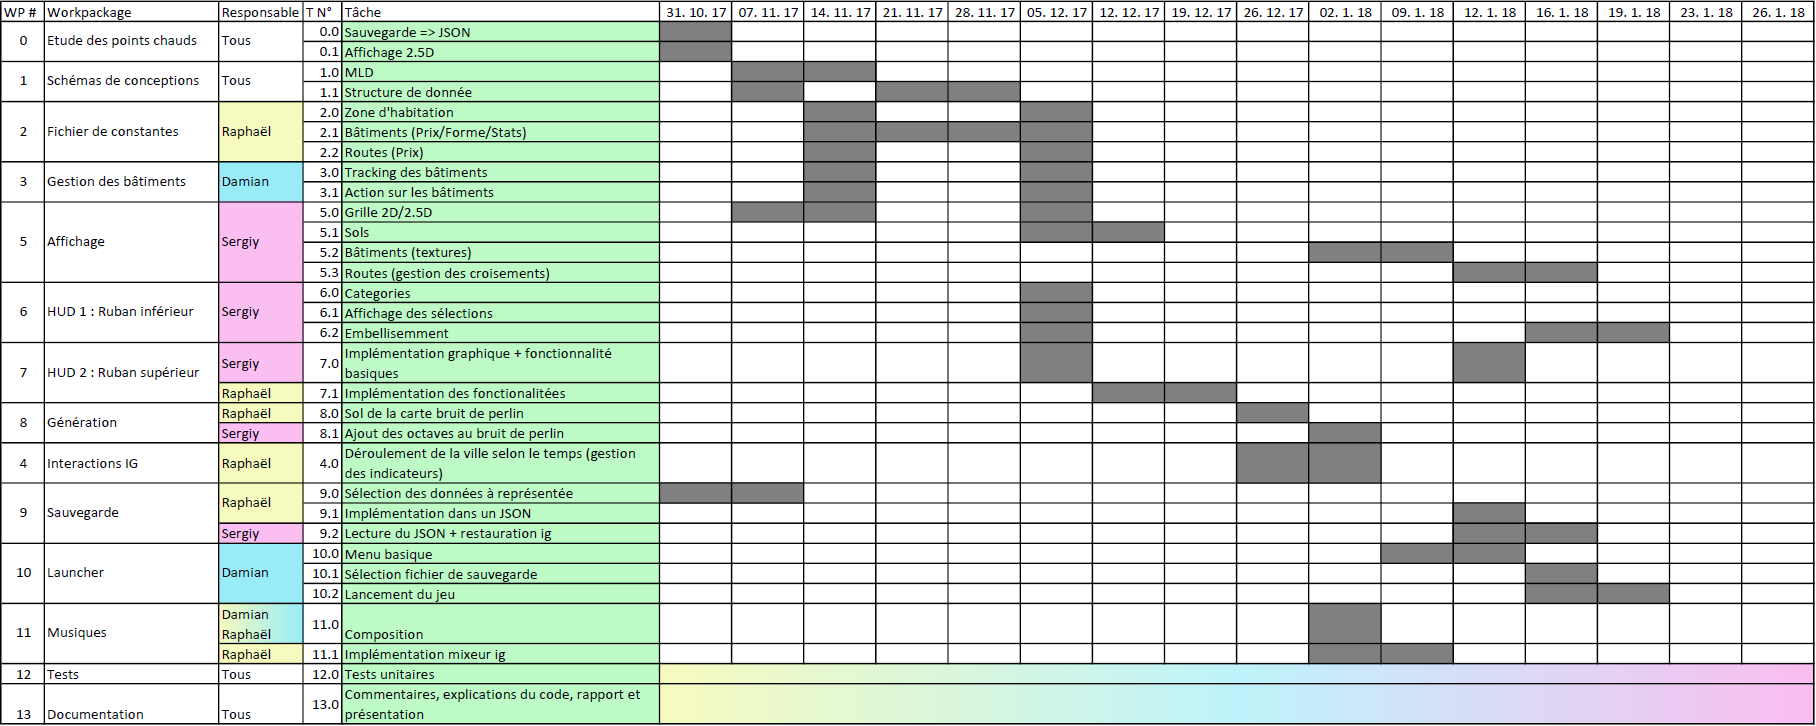
\includegraphics[width=1.1\textwidth]{img/planning_final.png}

\chapter{Conclusion}
\thispagestyle{headings}
Il est important de mentionner que notre but avant tout était de nous faire plaisir, ce pourquoi nous avons profité de la liberté de choisir notre projet en réalisant un jeu vidéo. Bien sûr, aucun de nous n'y jouera dans l'état dans lequel il est actuellement (il faut être honnête), mais nous sommes fiers de tout ce que nous avons appris sur le tas, et de la maturité que ce projet nous a apporté. En effet, nous avons désormais une bien meilleure idée de l'importance qu'a une bonne planification et une répartition des tâches intelligente.
\paragraph{}
L'organisation au sein d'un projet de groupe comme le P2 n'est pas une tâche facile car nous avons d'autres cours en parallèle dans des domaines totalement différents et sur lesquels nous avons l'obligation de travailler. Cela accentué par le fait que les personnes au sein d'un même groupe n'ont souvent pas la même façon de s'organiser face au reste des tâches scolaires et c'est précisément pour cela que la rigueur et la discipline que demande le travail en équipe nous a appris l'importance d'une bonne communication.
\paragraph{}
Nous somme heureux de nos progrès dans tous les domaines qui ont composé ce projet, en programmation bien sûr, mais pas seulement. Notre but a aussi été de profiter de l'occasion pour en apprendre plus sur des outils comme :
\begin{itemize}
\item git : Pour la gestion des fichiers du projet;
\item markdown : Pour la rédaction du wiki;
\item LaTeX : Pour la rédaction du présent rapport;
\item Et quelques autres encore.
\end{itemize}
\paragraph{}
Nous avons fait notre possible pour être "originaux" et sortir de l'ordinaire des projets scolaires en intégrant des fonctionnalités auxquelles nous n'avions jamais touchées, par exemple la 2.5D, la génération aléatoire d'environnements, l'intégration d'effets sonores, ou encore le principe de Launcher permettant de lancer une application avec une autre en ajoutant des paramètres d'entrée par exemple.

\chapter{Sources}
\begin{itemize}
\item Notre manuel de référence sur la programmation Qt a été basé sur le cours de 2017, intitulé "Programmation événementielle avec Qt 5" de notre école écrit par Messieurs Stéphane Beurret et David Grunenwald.
\item Pour le développement du projet en général, nous avons utilisé la documentation officiel en ligne du framework Qt : \url{http://doc.qt.io/}.
\item En ce qui concerne l'utilisation du bruit de Perlin, nous avons consulté une série de vidéo tutoriel en javascript (avec le framework p5) de la chaîne Youtube "the CodingTrain" par Daniel Shiffman qui a couvert le sujet : \url{https://www.youtube.com/user/shiffman}\\
Pour ce qui est de l'algorithme de Perlin (en lui même) utilisé, il a été trouvé sur le compte Github de Sol-program :
\url{https://github.com/sol-prog/Perlin_Noise}
\item Pour diverses spécificités liées à Qt qui n'étaient pas forcément évidentes de prime abord dans le cours de notre école ou dans la documentation officiel, nous avons profité à plusieurs reprise de l'expérience de la communauté du forum de Stack Overflow : \url{https://stackoverflow.com/}
\end{itemize}

\chapter{Annexes}
\thispagestyle{headings}
\end{document}